\documentclass[bwprint]{gmcmthesis}
\usepackage{amsmath}
\usepackage{pdfpages}
\usepackage{tikz}
\usetikzlibrary{shapes.geometric, arrows.meta, positioning}
\usepackage{algorithm}
\usepackage{algpseudocode} % 用于书写伪代码
\numberwithin{figure}{section}
\renewcommand{\thefigure}{\arabic{section}-\arabic{figure}} 
\usepackage{subcaption}
\usepackage{cite}  % 导入cite包以处理引用
 
\usetikzlibrary{calc}

%% 上下页边距设置为 2.5cm
\geometry{top=2.5cm,bottom=2.5cm}

\begin{document}

\begin{titlepage}

    \vspace*{1.5cm}
\begin{center}  
    {\Huge\bfseries 浙江大学第二十二届 \\ 大学生数学建模竟赛\par}  
\end{center}  

\vspace*{0.05cm}
\begin{center}
    {\normalsize\bfseries 2024 年 5 月 13 日 -5 月 22 日}
\end{center}

\vspace*{0.5cm}
\begin{center}
    {\Large\bfseries 团队名:\underline{ 模型肯定队 }}\par
    {\Large 题目:  $\;A$ \checkmark $\quad B$}  \par
    (在所选题目上打勾)
\end{center}

\vspace*{1cm}
\begin{center}
    \normalsize
    \begin{tabular}{|c|c|c|c|}
    \hline & 参赛队员 1 & 参赛队员 2 & 参赛队员 3 \\
    \hline 姓名 & 罗俊勋 & 谢锦川 & 王国兴 \\
    \hline 学号 & 3210101613 & 3210102597 & 3210105229 \\
    \hline 院 (系) & 数学科学学院 & \begin{tabular}{c} 
    航空航天学 \\
    院
    \end{tabular} & \begin{tabular}{c} 
    控制科学与 \\
    工程学院
    \end{tabular} \\
    \hline 专业 & 数学与应用数学 & 工程力学 & \begin{tabular}{c} 
    自动化(控制) 
    \end{tabular} \\
    \hline 手机 & 18174489027 & 15607000752 & 17789542605 \\
    \hline Email & junxun-luo@outlook.com & cattuft@outlook.com & 3210105229@zju.edu.cn  \\
    \hline
    \end{tabular}
\end{center}

\vspace*{2cm}
\begin{center}
    {\huge\bfseries 浙江大学本科生院}

    \par
    {\huge\bfseries 浙江大学数学建模实践基地}
\end{center}

\end{titlepage}


 %\maketitle
 \begin{abstract}
	无人机因其安全性、灵活性和可靠性等优点被广泛应用于搜索、勘探等领域。在实际应用中,往往需要多架无人机互相配合,协同工作以完成大规模大范围的搜索任务。然而,如何让多个无人机互相配合,高效准确地完成搜索任务是一个具有挑战性的问题。本文基于贪婪思想和区域划分等策略,提出了在两种不同场景下的无人机协同搜索方案。

   	对于搜索区域中目标数量和位置都未知的问题:关键在于如何合理地分配搜索任务,为此我们对目标区域进行划分并分配给对应的无人机;利用旋转搜索策略使无人机在其子区域内沿边界进行旋转搜索,从外向内逐步推进。此策略可以保证无人机在有限时间内最大程度地覆盖其负责的区域,增加发现目标的概率。
	
	对于目标区域中目标位置和权重已知的问题:利用\textbf{贪婪策略}给出总体路径趋势,再利用\textbf{路径局部优化}对路径进行微调,提高整体搜索效率,使得在规定时间内发现的目标权重之和最大化。
	
	本文所提出的方法通过合理的区域划分和优化策略,实现了对复杂搜索任务的有效解决,具有较高的实用价值。

	\keywords{\textbf{无人机协同搜索}\quad \textbf{凸包划分}\quad \textbf{边界搜索}\quad \textbf{贪婪策略}\quad \textbf{路径优化}}
\end{abstract}


% 正文
\section{问题背景和问题重述}

\subsection{问题背景}
无人机具有体积小、成本低、安全高效等优势,被广泛应用于搜索、勘探等领域。受限于体积、负载等原因,单架无人机完成复杂任务较为困难。协同区域搜索是指在满足环境和性能等多个约束条件下,为多架无人机规划搜索路径,并协调无人机之间的关系,确保无人机可以有效地执行区域搜索任务。\par

\subsection{问题重述}
基于上述背景,题目假定在地面上某个确定的待搜索区域内分布着 $M$ 个目标物,拟用 $N$ 架无人机协同完成搜索任务。无人机均在同一高度上飞行,无人机所在位置在地面的投影与某目标物距离不超过 $d$ 时视为发现该目标。本文将给出下面两种场景的求解方案\par
\begin{enumerate}
	\item 目标物的数量 $M$ 与位置均为未知。现要求在规定的任务时间 $T$ 内,发现目标物的数量尽可能多。
	\item 目标物的位置和权重均为已知。现要求在规定的任务时间 $T$ 内,发现目标物的权重之和尽可能大。
\end{enumerate}


\vspace*{1cm}
\section{模型假设与符号说明}
\subsection{模型假设}

	由于在实际应用中,区域 $D$ 的面积相对无人机搜索范围来说较大,因此我们取 $dx=dy=d$, 其中 $dx,dy$ 是坐标轴上的刻度。并用点 $(x_0,y_0)$ 被搜索代表区域 $\{(x,y):|x-x_0|\leq \frac{d}{2},|y-y_0|\leq \frac{d}{2}\}$ 被搜索,除此之外,对每一问题,做如下假设:

\subsubsection{问题一}
\begin{enumerate}
	\item 待搜索区域为凸包。
	\item 目标物随机分布在待搜索区域中。
	\item 每架无人机的飞行高度和飞行速度相同。
	\item 人为指定每架无人机的起飞位置。
\end{enumerate}

\subsubsection{问题二}
\begin{enumerate}
	\item 待搜索区域为矩形
	\item 目标物随机分布在待搜索区域中。
	\item 每架无人机的飞行高度和飞行速度相同。
	\item 所有无人机都从原点起飞。
\end{enumerate}

\subsection{符号说明}
$$
\begin{array}{c|l}
\hline \text { 符号 } & \text { 含义 } \\
\hline D & \text { 待搜索区域 } \\
d & \text { 无人机投影半径 } \\
L_x\times L_y & \text { 包围$D$的最小矩形 } \\
N & \text { 无人机数量 } \\
M & \text { 目标物数量 } \\
M' & \text { 最终搜索到的目标物数量 } \\
T & \text { 任务时间 } \\
v & \text { 无人机飞行速度 } \\
P_i(x_i,y_i) & \text { 目标物位置 } \\
w_i & \text { 目标物权重 } \\
S_{ij} & \text { $P_i$ 到 $P_j$ 的距离 } \\
S_{t} & \text { $t$ 时刻某无人机已经飞行的距离 } \\
S & \text { 最远飞行距离 }(=vT)\\
\hline
\end{array}
$$

\vspace*{1cm}
\section{模型建立与求解}

\subsection{问题一}
问题一未给定区域 $D$ 和目标物数量 $M$.不妨设区域 $D \subset L_x\times L_y = [0,l_x]\times [0,l_y]$。 现考虑 $M'$ 的值,记 $T$ 时刻所有无人机已经搜索的区域为 $D'$ ,则由模型假设,对充分大的 $M$ 最终搜索到的目标物数量满足下列关系
$$
\frac{M'}{M} = \frac{D'}{D}
$$
于是 $\max M' = M \max \frac{D'}{D} = \frac{M}{D} \max D' \sim \max D'$

问题转化为如何在给定的时间 $T$ 内,使得无人机搜索到的区域 $D'$ 最大。考虑到无人机速度恒定,且搜索时间给定。从而单个无人机的最大搜索范围由

$$
D'_{max} = 2dvT+\pi d^2
$$
给出 。

于是要使得 $D'$ 最大,只需使无人机之间搜索区域的重叠部分最小。于是将区域 $D$ 划分成 $N$ 个不同的子区域,每个无人机负责一个子区域的搜索。这使得不同无人机之间的搜索区域在空间上不交。

在考虑单个无人机的搜索时,采用边界旋转搜索策略。即无人机在其子区域内沿边界进行旋转搜索,这使得单个无人机的搜索区域在时间上不交。


\subsection{问题二}
对给定位置的的目标物,总存在 $L_x\times L_y$ 包含所有的点,于是可以给出每个点的位置 $P_i(x_i,y_i)$ 。假定所有无人机从原点出发,方便起见,记 $P_0(0,0),w_0 = 0$,并用序列 $\{path^j\},j=1,2,\cdots ,N$ 记录无人机 $j$ 的路径。先考虑第一个无人机,简记其路径为 $path$, 其递推公式由下式给出

1.  $path_0 = P_0= (0,0)$

2. 不妨设$path_l = P_i$,且此时无人机已经经过的距离为 $S_l$ ,则有

$$
temp_1 = \arg\max_{P_j}\left\{ \frac{w_j}{S_{ij}} :P_j\in \{P_1,P_2,\cdots,P_M\}\setminus \{path_i\}_{i=0}^{l},S_{ij}\leq S-S_l\right\}
$$
不妨设 $P_j = temp_1$(如果有),并记 $r_{ij} = \frac{w_j}{S_{ij}}$, 接下来做局部优化

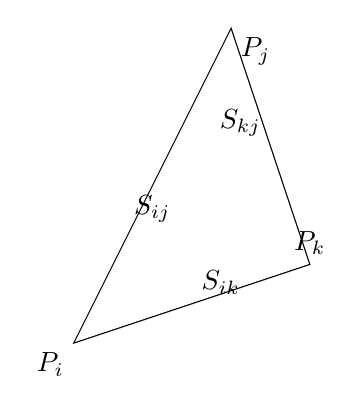
\begin{tikzpicture}  
    % Define the vertices of the triangle  
    \coordinate (P_i) at (0,0);  
    \coordinate (P_j) at (2,4);  
    \coordinate (P_k) at (3,1);  
      
    % Draw the triangle  
    \draw (P_i) -- (P_j) -- (P_k) -- cycle;  
      
    % Label the vertices  
    \node[below left] at (P_i) {$P_i$};  
    \node[below right] at (P_j) {$P_j$};  
    \node[above] at (P_k) {$P_k$};  
      
    % Label the sides  
    \node[below] at ($(P_i)!0.5!(P_j)$) {$S_{ij}$};  
    \node[above right] at ($(P_i)!0.5!(P_k)$) {$S_{ik}$};  
    \node[above left] at ($(P_j)!0.5!(P_k)$) {$S_{kj}$};  
\end{tikzpicture}  

取 
$$
temp_2 = \arg\max_{P_k}\left\{ \frac{w_k + w_j}{S_{ik} + S_{kj}} : S_{ik} + S_{kj} \leq S-S_l\right\}
$$
不妨设 $P_k = temp_2$(如果有), 并记 $r_{ikj} = \frac{w_k + w_j}{S_{ik} + S_{kj}}$

若 $r_{ikj} > r_{ij}$, 则 
$$
path_{l+1} = P_k,path_{l+2}=P_j,S_{l+2}=S_l+S_{ik}+S_{kj}
$$

否则 
$$
path_{l+1} = P_j,S_{l+1} = S_l + S_{ij}
$$

重复上述过程,直至无人机到达最大飞行距离或者所有点都被经过。

再对其他无人机执行上述过程,最终得到所有无人机的路径。


\vspace*{1cm}
\section{计算方法的设计}
\subsection{问题一}

\begin{center}
	\resizebox{0.4\textwidth}{!}{%
		\begin{tikzpicture}[node distance=2cm, auto, scale=0.4, transform shape]
			% Define style
			\tikzset{
				startstop/.style={rectangle, rounded corners, minimum width=3cm, minimum height=1cm, text centered, draw=black, fill=red!30},
				process/.style={rectangle, minimum width=3cm, minimum height=1cm, text centered, draw=black, fill=orange!30},
				decision/.style={diamond, aspect=2, text centered, draw=black, fill=green!30},
				arrow/.style={thick,->,>=stealth}
			}
			
			% Define blocks
			\node (start) [startstop] {初始化凸包和网格};
			\node (partition) [process, below of=start] {网格均匀划分为区域};
			\node (boundary) [process, below of=partition] {标记边界点};
			\node (move) [process, below of=boundary] {沿边界点移动};
			\node (store) [process, below of=move] {存储当前状态};
			\node (terminate) [decision, below of=store] {检查是否超时};
			\node (end) [startstop, below of=terminate, yshift=-0.5cm] {输出结果};
			
			% Define arrows
			\draw [arrow] (start) -- (partition);
			\draw [arrow] (partition) -- (boundary);
			\draw [arrow] (boundary) -- (move);
			\draw [arrow] (move) -- (store);
			\draw [arrow] (store) -- (terminate);
			\draw [arrow] (terminate) -- node[right] {是} (end);
			\draw [arrow] (terminate.east) -- ++(3,0) |- node[near start, right] {否} (boundary.east);
		\end{tikzpicture}%
	}
	\captionof{figure}{问题一解决方案算法流程图}
\end{center}



\subsubsection{Graham扫描法初始化凸包}


Graham \cite{graham1983finding} 扫描法通过维护一个候选点栈 \( S \) 来解决凸包问题。输入集 \( Q \) 中的每个点都被推入栈一次,非 \( CH(Q) \) 顶点的点最终被弹出栈。当算法终止时,栈 \( S \) 仅包含 \( CH(Q) \) 的顶点,且顶点按它们在边界上出现的逆时针顺序排列。

程序 \textbf{GRAHAM-SCAN} 接收点集 \( Q \) 作为输入,其中 \( |Q| \geq 3 \)。在不改变栈 \( S \)的情况下,调用函数 \textbf{Top}(\( S \)),返回栈 \( S \) 顶部的点,调用函数 \textbf{Next-To-Top}(\( S \)),返回栈 \( S \) 顶部下面一个条目的点\cite{10.5555/1614191}。

\begin{algorithm}
	\caption{计算凸包的 Graham 扫描算法}
	\begin{algorithmic}[1] % 可选参数 [1] 用于行号
		\State 设 $p_0$ 为点集 $Q$ 中 $y$ 坐标最小的点,
		\If{有多个这样的点}
		\State 则选择最左边的点。
		\EndIf
		\State 设 $(p_1, p_2, \dots, p_m)$ 为 $Q$ 中的其余点,
		\State 按照绕 $p_0$ 的极角逆时针顺序排序
		\If{多个点具有相同的角度}
		\State 只保留距离 $p_0$ 最远的那个点。
		\EndIf
		\State 将 $p_0$ 推入栈 $S$。
		\State 将 $p_1$ 推入栈 $S$。
		\State 将 $p_2$ 推入栈 $S$。
		\For{$i = 3$ \textbf{to} $m$}
		\While{由栈 $S$ 中的次顶点\textbf{Next-To-Top}($S$)、顶点\textbf{Top}($S$)和 $p_i$ 形成的角使得转向不是左转}
		\State 执行出栈(POP)操作。
		\EndWhile
		\State 将 $p_i$ 推入栈 $S$。
		\EndFor
		\State \Return 栈 $S$
	\end{algorithmic}
\end{algorithm}

\subsubsection{初始化网格和划分区域}
首先,算法初始化并生成一个覆盖特定区域的网格,然后判断每个网格点是否位于一个定义的凸包内部,并在相应位置更新一个矩阵标记有效区域。之后,删除该矩阵中的全零行和列,并进行边缘填充。算法计算每个区域应包含的点数,并通过迭代方式为每个区域分配网格点,直到每个区域的点数达到预定值。特别地,最后一个区域会被标记为特殊值,以确保覆盖完整。
\begin{algorithm}
	\caption{基于矩阵网格的区域划分算法}
	\begin{algorithmic}[1]
		\State 初始化网格点 $x, y$
		\State 生成网格 $xv, yv$
		\State 判断网格点是否在凸包内,存储结果于 $mask$
		\State 初始化全零矩阵 $matrix$
		\State 在 $mask$ 为真的位置将 $matrix$ 置为 $1$
		\State 删除 $matrix$ 中全零的行和列
		\State 对 $matrix$ 进行边缘填充
		\State 初始化用于记录的矩阵 $all\_matrix$
		\State 计算每个区域应含点数 $every\_drone\_point$
		\State 初始化 $last\_line$ 为 0
		
		\For{$index \gets 0$ \textbf{到} $plane\_nums-1$}
		\If{$index = plane\_nums - 1$}
		\State 将最后一个区域的点标记为特殊值
		\State \textbf{break}
		\EndIf
		\State 初始化当前无人机覆盖点数 $drone\_points \gets 0$
		\For{$line \gets last\_line$ \textbf{到} $\infty$}
		\State 遍历行内每个点,更新 $matrix$ 和 $drone\_points$
		\If{$drone\_points \geq every\_drone\_point$}
		\State 更新 $last\_line$ 并跳出内层循环
		\EndIf
		\EndFor
		\EndFor
	\end{algorithmic}
\end{algorithm}


\subsubsection{无人机绕边界旋转搜索}
首先,初始化一个包含无人机标识和辅助值的列表。之后,循环地进行边界检测:判断矩阵中元素是否属于无人机,进而识别和标记每架无人机的边界点。将边界点按与质心的角度排序。一旦所有边界确定,更新矩阵中的边界点状态。

\begin{algorithm}
	\caption{无人机边界检测和移动过程}
	\begin{algorithmic}[1]
		\State 初始化无人机标识列表 $number\_list$,并添加辅助边界值 $0$ 和 $2$
		\State 输出 $number\_list$
		\While{矩阵中存在除 $0$ 和 $2$ 之外的元素}
		\State 初始化边界列表 $bounds$ 为空,计数器 $counter$ 设为 $0$
		\For{每架无人机标识 $index$}
		\State 初始化边界 $bound$ 为空列表
		\State 从 $number\_list$ 移除当前无人机标识符
		\For{矩阵的每个元素 $(i, j)$}
		\If{元素标识为 $index$ 且周围含有其他标识}
		\State 添加 $(i, j)$ 到 $bound$
		\State 将 $(i, j)$ 处矩阵元素设置为 $3$
		\EndIf
		\EndFor
		\State 将 $index$ 添加回 $number\_list$
		\State 对 $bound$ 按角度排序并添加到 $bounds$
		\EndFor
		\If{$bounds$ 为空}
		\State 输出 $bounds$ 并退出循环
		\EndIf
		\While{True}
		\If{所有 $bounds$ 的最大长度 $\leq counter$}
		\State 退出循环
		\EndIf
		\For{每个 $bound$}
		\If{$bound$ 的长度 $> counter$}
		\State 将对应矩阵位置设置为 $2$
		\EndIf
		\EndFor
		\If{$counter$ 是采样频率的倍数}
		\State 记录当前矩阵状态
		\EndIf
		\State $counter$ 自增 $1$
		\If{总运行时间超过最大时间}
		\State 退出循环
		\EndIf
		\EndWhile
		\If{总时间超过最大时间}
		\State 退出循环
		\EndIf
		\EndWhile
	\end{algorithmic}
\end{algorithm}

\subsubsection{问题一求解结果}

\begin{enumerate}
	\item 实例一:4架无人机进行搜索,指定点为[100,300],[400, 0], [900, 0], [200, 500]。
	\begin{figure}[h]
		\centering
		\begin{subfigure}{0.5\textwidth}  % 增加宽度比例以适应放大的图像
			\centering
			\includegraphics[width=\textwidth]{../assets/img/1.png}  % 这里仍然使用\textwidth,因为subfigure的宽度已经调整
			\caption{区域划分}
		\end{subfigure}\hfill
		\begin{subfigure}{0.5\textwidth}  % 同上,调整宽度比例
			\centering
			\includegraphics[width=\textwidth]{../assets/img/2.png}  % 保持宽度与subfigure一致
			\caption{无人机搜索}
		\end{subfigure}
		\caption{问题一实例一可视化结果}
	\end{figure}
	\vspace{1cm} % 在此处调整间距
	\item 实例二:5架无人机进行搜索,指定点为[100,300],[600, 0], [900, 0], [200, 800]。
		\begin{figure}[h]
		\centering
		\begin{subfigure}{0.5\textwidth}  % 增加宽度比例以适应放大的图像
			\centering
			\includegraphics[width=\textwidth]{../assets/img/3.png}  % 这里仍然使用\textwidth,因为subfigure的宽度已经调整
			\caption{区域划分}
		\end{subfigure}\hfill
		\begin{subfigure}{0.5\textwidth}  % 同上,调整宽度比例
			\centering
			\includegraphics[width=\textwidth]{../assets/img/4.png}  % 保持宽度与subfigure一致
			\caption{无人机搜索}
		\end{subfigure}
		\caption{问题一实例二可视化结果}
	\end{figure}
\end{enumerate}

\subsubsection{问题一结果分析}

	程序的运行结果表明,我们的算法能够有效地将搜索区域划分为不同的子区域,并通过边界搜索策略,使得无人机在有限时间内最大程度地覆盖其负责的区域,增加发现目标的概率。


\subsection{问题二}

\begin{center}
	% Define styles for the flowchart
	\tikzstyle{startstop} = [rectangle, rounded corners, minimum width=3cm, minimum height=1cm, text centered, draw=black, fill=red!30]
	\tikzstyle{process} = [rectangle, minimum width=3cm, minimum height=1cm, text centered, draw=black, fill=orange!30]
	\tikzstyle{decision} = [diamond, aspect=2, text centered, draw=black, fill=green!30]
	\tikzstyle{arrow} = [thick,->,>=stealth]
	
	\begin{tikzpicture}[node distance=2cm, auto, scale=0.7, transform shape]
		\node (init) [startstop] {初始化参数};
		\node (generate) [process, below of=init] {生成搜集点};
		\node (assign) [process, below of=generate] {无人机路径规划};
		\node (inLoop) [process, below of=assign, yshift=-0.5cm] {排序搜集点};
		\node (decision1) [decision, below of=inLoop, yshift=-0.5cm] {有可达点吗?};
		\node (update) [process, below of=decision1, yshift=-0.5cm] {选择最优点,更新路径};
		\node (check) [decision, below of=update, yshift=-0.5cm] {飞行距离 $S_i < S$?};
		\node (stop) [startstop, below of=check, yshift=-0.5cm] {计算总收益};
		
		% Arrows
		\draw [arrow] (init) -- (generate);
		\draw [arrow] (generate) -- (assign);
		\draw [arrow] (assign) -- (inLoop);
		\draw [arrow] (inLoop) -- (decision1);
		\draw [arrow] (decision1) -- node[right] {是} (update);
		\draw [arrow] (update) -- (check);
		\draw [arrow] (check.west) -- ++(-2,0) |- node[near start, left] {是} (assign.west);
		\draw [arrow] (check) -- node[right] {否} (stop);
		\draw [arrow] (decision1.east) -- ++(3,0) |- node[near start, right] {否} (inLoop.east);
	\end{tikzpicture}
	\captionof{figure}{问题二解决方案算法流程图}
\end{center}

\subsubsection{初始化参数与生成搜集点}
设置搜索区域的长 $X$ 和宽 $Y$ 、无人机数量 $N$ 、目标物数量 $M$ 、最远飞行距离 $S$ 、最大权$W_{max}$ 和最小权 $W_{min}$ 。


\subsubsection{无人机路径规划算法}
假定有 $N$ 个无人机, $M$ 个点(对应区域),设点 $P_i$ 到 $P_j$ 的距离为 $S_{ij}$,点 $P_i$ 的权为 $W_i$。对于每个无人机,记原点为 $P_i$ ,首先计算路径均分下权重最高的点 $P_j$ ,即 $\max \left\{ \frac{W_j}{S_{ij}} : \forall j \right\}$ 对应的点($j$不包括$i$)。再计算当前状态下收益最高的点 $P_k$ ,即 $\max \left\{ \frac{W_k + W_j}{S_{ik} + S_{kj}} : \forall k \right\}$ 对应的点($k$不包括$i, j$)。由计算公式已知,$\left\{ \frac{W_k + W_j}{S_{ik} + S_{kj}} : \forall k \right\}$ 对应点集中若存在点对应的 $\frac{W_k + W_j}{S_{ik} + S_{kj}} > \frac{W_j}{S_{ij}}$ ,则路径选取为$ P_i \rightarrow P_k \rightarrow P_j $,再将起点 $P_i$ = $P_j$ ,重复上述操作,直至点都被经过或到达最大飞行时间。

\begin{algorithm}
	\caption{无人机路径规划算法}
	\begin{algorithmic}[1]
		\For{each UAV}
		\State 从原点出发,设起点为 $P_i$
		\While{未到达最大飞行时间且有未访问点}
		\State 计算 $P_i$ 到除 $P_i$ 其他所有点的效益 $r_i$
		\State 选择效益 $r_i = \max \left\{ \frac{W_j}{S_{ij}} : \forall j \right\}$ 最大的点记为 $P_j$
		\State 计算到除 $P_i$, $P_j$ 其他所有点的效益 $r_i'$
		\State 选择效益 $r_i' = \max \left\{ \frac{W_k + W_j}{S_{ik} + S_{kj}} : \forall k \right\}$ 最大的点记为 $P_k$
		\State 将路径更新为 $P_i \rightarrow P_k \rightarrow P_j$
		\State 令起点 $P_i = P_j$
		\EndWhile
		\EndFor
	\end{algorithmic}
\end{algorithm}

\subsubsection{计算总收益}
计算两种情况下的总收益。首先,对所有点的权重求和,得到假设所有点都被搜索到时的总收益。然后,对无人机实际访问到的点的权重求和,计算实际搜索到的总收益。

\subsubsection{问题二求解结果}
\begin{enumerate}
	\item 实例一:3架无人机进行搜索,目标物共70个,待搜索区域为 $ 300*200 $ 的矩形,最远飞行距离为700,最小权为10,最大权为100。
	
	\begin{figure}[h]
		\centering
		\includegraphics[width=\textwidth]{../assets/img/5.png}  % 这里将图像宽度设为页面宽度的一半
		\caption{问题二实例一可视化结果}
	\end{figure}
	
	%\vspace{1cm} % 在此处调整间距
	\item 实例二:5架无人机进行搜索,目标物共700个,待搜索区域为 $ 3000*2000 $ 的矩形,最远飞行距离为10000,最小权为10,最大权为100。
	
	\begin{figure}[h]
		\centering
		\includegraphics[width=\textwidth]{../assets/img/6.png}  % 这里将图像宽度设为页面宽度的一半
		\caption{问题二实例二可视化结果}
	\end{figure}

\subsubsection{问题二结果分析}
	程序结果表明,基于贪婪策略的路径规划能够显著提高搜索效率,使得无人机在有限时间内搜索到的目标物权重之和最大。此外,通过路径局部优化,进一步提升了搜索效率。我们在实验中加入了路径微调机制,确保无人机能够动态适应环境变化,从而避免路径重叠和不必要的绕行。

\end{enumerate}

\vspace*{1cm}
\section{模型评价与展望}
\subsection{模型评价}
\begin{enumerate}
	\item 本文提出的多无人机协同搜索模型,通过区域划分和贪婪策略,实现了在规定时间内最大化目标物品权重的搜索效率。在两个不同场景下(目标数量和位置未知以及目标位置和权重已知)均取得了较好的效果。
\end{enumerate}
	

\subsection{工作展望}
\begin{enumerate}
	\item 当前的区域划分方法是静态的,即在任务开始前预先划分。引入动态区域划分方法,可以根据无人机实时反馈的搜索进展和目标密度调整子区域的边界,提高搜索的灵活性和效率
	\item 除了边界旋转搜索策略,可以引入其他搜索策略(如随机搜索、基于梯度的搜索等)并结合机器学习算法,使得无人机可以根据环境和目标分布动态选择最优策略
	\item 增强无人机之间的通信与协同决策能力,使得它们可以实时共享信息并协同调整搜索路径,避免重复覆盖和资源浪费,提高整体搜索效率。
\end{enumerate}


%参考文献
\newpage
\section{参考文献}
\bibliographystyle{plain}
\bibliography{reference}

\newpage
%附录
\appendix
\section{问题一程序代码}
\begin{lstlisting}[language=Python] 
	import numpy as np
	np.set_printoptions(threshold=np.inf)
	import matplotlib.pyplot as plt
	from scipy.spatial import ConvexHull
	from matplotlib import path, animation
	import itertools
	
	#*******************************************************
	###############参数#####################################
	n = 1000    # 定义矩阵大小(根据实际情况,n=max {[L_x/d], [L_y/d]})
	plane_nums = 5  #无人机数量
	MaxTime = 3000  #最大时间
	totaltime = 0   #初始化当前用时
	speed  = 30   #无人机速度 (d*m/s)
	frequence =500  #图像采样频率
	points = np.array([[100,900],[800, 0], [900, 950], [400, 10]])  # 指定区域边界
	output = "多架无人机搜索过程.gif" #输出文件名
	
	#*******************************************************
	# 对这些点创建凸包
	hull = ConvexHull(points)
	
	# 创建网格点
	x = np.arange(n)
	y = np.arange(n)
	xv, yv = np.meshgrid(x, y)
	
	# 检查网格中的每个点是否在凸包内
	path_points = path.Path(points[hull.vertices])
	mask = path_points.contains_points(np.vstack([xv.flatten(), yv.flatten()]).T)
	mask.shape = xv.shape
	
	# 根据 mask 创建一个全零矩阵,并在 mask 为 True 的地方置为 1
	matrix = np.zeros((n, n))
	matrix[mask] = 1
	
	# 删除全零行和全零列
	matrix = matrix[~np.all(matrix == 0, axis=1)]
	matrix = matrix[:, ~np.all(matrix == 0, axis=0)]
	
	matrix = np.pad(matrix, pad_width=1, mode='constant', constant_values=0)
	
	
	# 创建一个用于记录搜索轨迹的矩阵
	#matrix_trace = matrix.copy()
	all_matrix = []
	
	#分割
	#计算每个区域的点数
	every_drone_point = len(np.argwhere(matrix == 1)) / plane_nums
	last_line = 0
	
	for index in range(plane_nums):
		if index == plane_nums - 1:
			last = np.argwhere(matrix == 1)
			matrix[last[:, 0], last[:, 1]] = 10*(index + 1)
			break
	
		drone_points = 0
		for line in range(last_line, 9999999):
			for i, j in itertools.product(range(matrix.shape[0]), range(min(line, matrix.shape[1]))):
				if matrix[i, j] == 1:
					drone_points += 1
					matrix[i, j] = 10*(index + 1)
	
			if drone_points >= every_drone_point:
				last_line = line
				break
	
	
	#搜索
	
	number_list = [ 10*(index+1) for index in range(plane_nums)]
	number_list.append(0)
	number_list.append(2)
	
	print(number_list)
	while np.any((matrix != 0) & (matrix != 2)):
		#print(111)
		bounds = []
		counter = 0 #计数采样频率
	
		#对每架无人机赵边界
		for index in range(plane_nums):
			bound = []
			number_list.remove(10*(index+1))
			#每个的边界搜索
			for i in range(0, matrix.shape[0] - 1):
				for j in range(0, matrix.shape[1] - 1):
					#if matrix[i][j] == 1:
					if \
						(matrix[i][j] == 10*(index + 1)) and \
						(matrix[i - 1][j] in number_list or matrix[i + 1][j] in number_list or matrix[i][j - 1] in number_list or matrix[i][j + 1] in number_list) :
						bound.append([i, j])
						matrix[i,j] = 3
			number_list.append(10*(index+1))
	
			bound = np.array(bound)
			if bound.size != 0:
				bound = bound[np.argsort(np.arctan2(bound[:,1] - np.mean(bound[:,1]), bound[:,0] - np.mean(bound[:,0])))]
			else:
				bound = np.array(bound).reshape(-1, 2)
			bounds.append(bound)
		
		#若所有边界都为空,则跳出循环
		condition = 0
		for index in range(plane_nums):
			if bounds[index].size != 0:
				condition = 1
		
		if condition == 0:
			print(bounds)
			break
	
		#开始遍历
		while(True):
	
			if max(len(i) for i in bounds) <= counter:
				break
	
			for bound in bounds:
				#该边界已遍历完
				if len(bound) <= counter:
					pass
				else:
					i, j =bound[counter]
					matrix[i,j] = 2
			
			if counter % frequence == 0:
				all_matrix.append(matrix.copy())
	
			counter += 1
			#print(matrix)
			totaltime += 1.0 / speed
	
			if totaltime > MaxTime: #超时
				break
	
		if totaltime > MaxTime: #超时
				break
	
	
	print("===================================================")
	print("无人机速度:{:.2f}".format(speed))
	print("总用时:{:.2f}".format(totaltime))
	print("仿真完成,正在生成动态图像,过程可能较长,请稍等")
	# 使用自定义颜色映射来改变颜色,0为黑色,1为白色,表示待搜索区域,2为绿色(表示已搜索区域)
	cmap = plt.cm.colors.ListedColormap(['black', 'white', 'green', 'blue', "yellow", "purple", "grey", "pink", "lightblue", "c", "teal"])
	bounds=[-2, 0.5, 1.5, 2.5, 3.5, 11, 21, 31, 41, 51, 61, 71]
	norm = plt.cm.colors.BoundaryNorm(bounds, cmap.N)
	
	
	def animate(frame):
		ax.clear()
		im = ax.imshow(all_matrix[frame], cmap=cmap, norm=norm, origin='lower')
		return [im]
	
	# 创建动画
	fig, ax = plt.subplots(figsize=(8, 8))
	ani = animation.FuncAnimation(fig, animate, frames=len(all_matrix), interval=5, blit=True)
	
	# 保存动画
	ani.save(output, writer='pillow')
	
	# 显示动画
	plt.show()
	
\end{lstlisting}

\appendix
\section{问题二程序代码}
\begin{lstlisting}[language=Python] 

	# 生成区域中 M 个 权重为 W_i 的搜集点
	import random as rd
	import numpy as np
	import matplotlib.pyplot as plt
	from copy import deepcopy
	from matplotlib import pyplot as plt
	# plt.rcParams['font.sans-serif']=['SimHei'] #用来正常显示中文标签
	plt.rcParams['axes.unicode_minus']=False #用来正常显示负号
	
	# 计算两点之间的距离
	def distance(a, b):
		return np.sqrt((a[0] - b[0]) ** 2 + (a[1] - b[1]) ** 2)
	
	# 计算 W_i/S_ij, 给出排序后的列表
	def sort_map(p_i,map):
		return sorted(map,key=lambda x: x[-1]/distance(p_i,x[0:2]),reverse=True)
	
	#*******************************************************
	###########################参数#########################
	m, n = 3000, 2000 # 区域大小 单位:米
	M = 700 # 搜集点数量 
	N = 5  # 无人机数量
	S = 10000 # 设置最远飞行距离 单位:米
	max_W, min_W = 100, 10 # 设置权上下限 
	########################################################
	
	points = [[rd.randint(0, m), rd.randint(0, n),rd.randint(min_W,max_W)] for _ in range(M)]
	copy_points = deepcopy(points)
	
	# 路径
	
	paths = []
	
	for _ in range(N):
		path = [[0,0]] # 第 i 个无人机的路径
		temp_map = deepcopy(points)
		S_i = 0
		p_i = [0,0] # 起始点都设置成(0,0)
	
		while S_i < S:
	
			# 得到权重排序的序列
			sorted_map = sort_map(p_i,temp_map)
	
			# 如果所有剩下的距离都大于 S-S_i,则退出
			if all(distance(p_i, p) > S-S_i for p in sorted_map):
				break
			 
			# 优先选择权重大的
			for point in sorted_map:
				dis_pi_to_point = distance(p_i,point)
				if dis_pi_to_point < S - S_i:
					path.append(point)
					# 从 pi开始
					p_i = point
					S_i += dis_pi_to_point
					# 删掉这个点
					temp_map.remove(point)
					points.remove(point) # 下一个无人机不能经过这个点
					break
				else:
					continue
			
		
		paths.append(path)
	
	# 将所有点的权重相加就是全部搜索完的总收益
	total_gain_all = sum([point[2] for point in copy_points])
	print("全部搜索完的总收益:", total_gain_all)
	
	# 无人机实际访问到的所有点的权重之和就是搜索到的总收益
	total_gain_found = sum([point[2] for path in paths for point in path if len(point) > 2])
	print("搜索到的总收益:", total_gain_found)
	
	print("============================")
	print("搜索完成,搜索结果:")
	print("若全部搜完的总收益:", total_gain_all)
	print("实际的总收益:", total_gain_found)
	print(f"收益率:{total_gain_found / total_gain_all:.2%}")
	
	# 假设 paths 是一个包含多个路径的列表,每个路径是一个点的列表,例如 [[(x1, y1), (x2, y2), ...], [(x1, y1), (x2, y2), ...], ...]  
	
	# 绘制点
	fig, ax = plt.subplots(figsize=[10, 6])  # 调整画布大小
	color_list = ['b', 'g', 'r', 'c', 'm', 'y', 'k']  # 颜色列表,为了区分不同无人机的路径
	
	for i, path in enumerate(paths):
		x_values = [point[0] for point in path]
		y_values = [point[1] for point in path]
		plt.plot(x_values, y_values, marker='o', linewidth=2, linestyle='-', color=color_list[i%7])  # 使用不同颜色
	
	# 标记未访问点
	for point in copy_points:
		x, y, weight = point
		plt.scatter(x, y, marker='x', color='k')  # 使用不同标记和颜色
		plt.annotate(f'{weight}', (x, y), textcoords="offset points", xytext=(0,10), ha='center')
	
	# 添加标题和标签
	plt.title('Drone Paths')
	plt.xlabel('X')
	plt.ylabel('Y')
	
	# 添加理论收益,实际收益及收益率
	total_gain_all = sum([point[2] for point in copy_points])
	total_gain_found = sum([point[2] for path in paths for point in path if len(point) > 2])
	revenue_rate = total_gain_found / total_gain_all
	props = dict(boxstyle='round', facecolor='wheat', alpha=0.5)
	
	info_text = f'expected: {total_gain_all}   actual: {total_gain_found}   ratio: {revenue_rate:.2%}'
	plt.text(0.12, 1.05, info_text, transform=ax.transAxes, fontsize=12, horizontalalignment='center', verticalalignment='top', bbox=props)
	
	plt.show()

\end{lstlisting}

\end{document} 
